%!TEX TS-program = pdflatex
%!TEX encoding = UTF-8 Unicode
%!TeX spellcheck = it_IT
%!TEX root = ../tesi.tex
%
\chapter{\textit{Obstacle Shadowing Model}}
%
\section{Il modello matematico}
Gli autori di~\cite{Carpenter:2015:OMI:2756509.2756512} riprendono il modello introdotto da Christoph Sommer et al.\ in~\cite{5720204},
nel quale la perdita di segnale dovuta a ostacoli $L_{s,o}$ dipende dall'attenuazione causata dai bordi dell'ostacolo (\textit{per-wall attenuation})
e quella derivante dalla superficie interna (\textit{per-meter attenuation}):
\begin{gather}\label{eq:osbtacle-model}
	L_{s,o} = \alpha n + \beta d_o
\end{gather}
Nella formula precedente, $n$ indica il numero di volte che il bordo dell'ostacolo viene intersecato dalla visuale (of LoS, da \textit{Line of sight}),
mentre $d_o$ è la distanza, in metri, attraversa all'interno dell'ostacolo.
Il parametro $\alpha$ rappresenta l'attenuazione per-metro espressa in decibels (dBm), invece
$\beta$ l'attenuazione per-metro, sempre in decibels (dB/m).

I due fattori di calibrazione permettono di rappresentare più tipologie di edificio.
I valori predefiniti di $\alpha = 9$ dBm e $\beta = 0,4$ dB/m sono buoni per la maggior parte delle applicazioni
anche se, naturalmente, non per tutte.
Riportando l'esempio in~\cite{5720204} di una casa in costruzione, il modello riesce a rappresentare le caratteristiche dell'attenuazione,
tuttavia i parametri sono distanti da quelli sopra indicati: $\alpha$ = 2.4 dBm and $\beta$ = 0.63 dB/m.
%
\begin{figure}[!h]
	\centering
	\begin{center}
		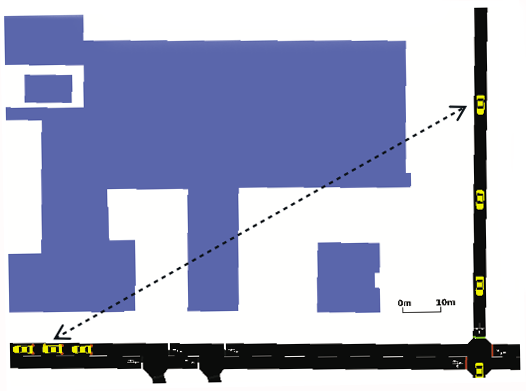
\includegraphics[width=.8\textwidth]{carpenter-1.png}
	\end{center}
	\label{fig:scenario-urbano-1}\caption{Esempio di scenario urbano.}
\end{figure}
%
Prendiamo l'esempio raffigurato in Figura~\ref{fig:scenario-urbano-1}, dove la linea fra i due veicoli interseca $n=6$ muri e una distanza interna di $d_o=32$m;
sostituendo i valori in~\ref{eq:osbtacle-model} si ottiene: $L_{s,o} = 9*6 + 0,4*32 = 66,8$dB.
Si evince come, con questa quantità di attenuazione, sia difficile che la trasmissione da un veicolo abbia abbastanza potenza per essere ricevuta dal secondo veicolo.
%
\section{L'implementazione}
Nel dettaglio, gli ostacoli sono rappresentati da poligoni bidimensionali che ne definiscono i bordi (spigoli).
Riprendendo l'esempio in Figura~\ref{fig:scenario-urbano-1}, la linea di visibilità (in questo caso \textit{obstructed-line-of-sight}, OLOS), fra i due veicoli potrebbe
intersecare diversi muri e percorrere una certa distanza internamente a uno o più edifici.
Il modello \textit{Obstacle Shadowing} conta il numero di intersezioni con gli spigoli dell'ostacolo, calcola la distanza percorsa internamente a esso e, utilizzando
il modello matematico visto in precedenza, restituisce l'attenuazione della trasmissione wireless fra i due veicoli.

Il tutto è implementato in ns-3 tramite tre classi: \textsf{Obstacle} contiente la rappresentazione geometrica dell'ostacolo, utilizzando le Computational Geometry Algorithms Library (CGAL),
come anche i parametri dell'attenuazione per-metro e per-muro.
\textsf{Topology} legge i dati degli edifici da un file specifico, generato dall'utility Polyconvert del software SUMO (Simulator for Urban Mobility)~\cite{sumoWebsite}
a partire dalle informazioni ottenute da OpenStreetMap (OSM)~\cite{osmWebsite}.
L'oggetto \textsf{Topology} così creato è poi utilizzato per determinare la perdita di segnale fra due punti (e.g. veicoli), utilizzando l'Algoritmo~\ref{algo:algoritmo-getobstucteddistancebetween}.
%
\begin{algorithm}[!h]
\caption{Algoritmo per determinare il numero di intersezioni con i bordi dell'ostacolo e la distanza interna percorsa fra due punti.}\label{algo:algoritmo-getobstucteddistancebetween}
\begin{algorithmic}[1]
	\Procedure{GetObstuctedDistanceBetween}{$p_1, p_2, B$}
	\BState{}\emph{Input}: $p_1, p_2$: posizione dei due veicoli; $B$: partizione binaria dello spazio (BSP) di ostacoli.
	\BState{}\emph{Output}: Distanza interna percorsa, $m_o$, e il numero di intersezioni con i bordi, $n$.
	\State{$m_o \gets 0;\; n \gets 0$}
	\TextState{Inizializza la portata massima $r$: distanza dal punto $p_1$ o $p_2$ al centro di un ostacolo, utilizzata per filtrare il sottoinsieme di ostacoli sufficientemente vicini.}
	\TextState{Crea un riquadro di delimitazione $b$ per $p_1$ e $p_2$ ed estendila di $r$ in tutte le direzioni.}
	\TextState{Calcola l'insieme di potenziali ostacoli $O$ da quelli all'interno di $b$ in $B$.}
	\ForEach{ostacolo $o \in O$}
		\If{(distance($p_1$, o.center) $< r$) OR (distance($p_2$, o.center) $< r$)}
			\ForEach{spigolo $e \in o$}\label{algo:line:getobstucteddistancebetween-interesezione}
				\If{$s$ interseca un raggio da $p_1$ a $p_2$}
					\State{$n \gets n+1$}
					\TextState{Salva la distanza minima e massima da $\{ p_1, p_2\}$ al punto d'intersezione.}
				\EndIf{}
				\TextState{$m_o \gets m_o+$ differenza fra i valori min e max calcolati al passo precedente.}
			\EndFor{}
		\EndIf{}
	\EndFor{}
	\Return{$m_o$ e $n$}
	\EndProcedure{}
\end{algorithmic}
\end{algorithm}
%
\section{Estensione a tre dimensioni}
Come detto in precedenza, gli oggetti sono rappresentati da poligoni bidimensionali e, conseguentemente,
il modello descritto lavora in una proiezione bidimensionale dell'ambiente (tridimensionale) di ns-3,
prendendo quindi in considerazione solo le prime due componenti \textit{x} e \textit{y} della posizione di ogni nodo.

Uno dei principali motivi che portò gli ideatori del modello a questa scelta fu la mancanza di informazioni tridimensionali
su OSM (piattaforma dalla quale aquisivano i dati), soprattutto su larga scala.
Nonostante in parte sia vero anche attualmente (spacialmente per aree rurali), queste informazioni sono sicuramente
più diffuse rispetto ad alcuni anni fa e lo saranno sempre di più.

Dato, quindi, il supporto nativo alla terza dimensone di ns-3 (a differenza dei suoi precedessori) e la crescente diffusione
di dati trimensionali sugli edifici in ambienti urbani e suburbani, è naturale pensare di estendere il modello affinché
tenga conto di questa componente e pertanto dell'esatta posizione del nodo nell'ambiente della simulazione.
%
\subsection{Altezza degli edifici}
Sebbene le forma degli edifici si possa descrivere esclusivamente in due dimensioni (punti bidimensionali che ne delineano il perimetro al suolo),
OSM prevede la possibilità di definire l'altezza totale in metri e/o specificare il numero di piani (sopra e sotto il livello del suolo)
presenti.
Questa informazione può essere sfruttata per creare una forma tridimensionale semplificata dell'edificio.
%
\begin{lstlisting}[language=XML,style=mystyle,linewidth=\textwidth,label={lst:esempio-dati-blocco-torre},caption={Esempio di informazioni di un edificio estratte da OSM.}]
<way id="62332429" visible="true" version="13" changeset="44057933" timestamp="2016-11-30T11:53:34Z" user="Agno-phi" uid="731498" >
 <nd ref="778692594"/>
 <nd ref="778692588"/>
 <nd ref="778692589"/>
 <nd ref="1809913218"/>
 <nd ref="778692593"/>
 <nd ref="778692594"/>
 <tag k="addr:city" v="Padova"/>
 <tag k="addr:housenumber" v="63"/>
 <tag k="addr:postcode" v="35121"/>
 <tag k="addr:street" v="Via Trieste"/>
 <tag k="alt_name" v="Torre Archimede;Tullio Levi Civita"/>
 <tag k="amenity" v="university"/>
 <tag k="building" v="university"/>
 <tag k="building:levels" v="8"/>
 <tag k="building:levels:underground" v="2"/>
 <tag k="name" v="Dipartimento di Matematica 'Tullio Levi-Civita'/>
 <tag k="operator" v="Universita' degli Studi di Padova"/>
 <tag k="website" v="http://www.math.unipd.it/"/>
</way>
\end{lstlisting}
%
Nell'esempio indicato in Figura~\ref{lst:esempio-dati-blocco-torre}, manca la misura dell'altezza ma è presente
il numero di piani: è sufficiente moltiplicare questo numero, qui $8$, per l'altezza media un piano, per esempio $2,7$ metri,
per ottenere una stima dell'altezza pari a $21,6$ metri.
Questo calcolo è stato incluso in uno \textit{script}\footnote{\url{https://gitlab.com/mromanelli/tesi}.} creato appositamente per integrare i dati sulle altezze nel file
dei poligoni generati dall'utility Polyconvert.
%
\begin{lstlisting}[language=XML,style=mystyle,linewidth=\textwidth,label={lst:esempio-poly-blocco-torre},caption={Forma di un edificio estratta da OSM e convertita con Polyconvert con l'aggiunta dell'altezza.}]
<poly id="62332429" type="amenity.university" color="237,199,199" fill="1" layer="-1.00" height="21.6" shape="79.68,73.38 119.66,61.39 108.52,24.49 88.84,30.39 68.53,36.48 79.68,73.38" />
\end{lstlisting}
%
\subsection{Modifica dell'algoritmo}
Il resto dell'algoritmo \textsf{GetObstuctedDistanceBetween} (Figura~\ref{algo:algoritmo-getobstucteddistancebetween})
rimane sostanzialmente lo stesso e, nello specifico, la ricerca dei potenziali ostacoli rimane invariata.
Infatti gli ostacoli che si interpongono fra due punti nello spazio tridimensionale saranno gli stessi che sul piano bidimensionale
(creato dalla perdita della terza componente \textit{z}) in quanto gli ostacoli che vengono considerati sono "ancorati" al terreno ($z=0$).
Anche l'oggetto \textsf{Obstacle} rimane quasi del tutto invariato, fatta eccezione per il valore l'altezza.

Le modifiche significative risiedono quasi totalmente nel calcolo delle intersezioni fra l'ostacolo e il raggio che collega i due nodi.
In origine, l'intersezione veniva calcolata fra il segmento (raggio) che unisce i due punti e lo spigolo dell'ostacolo considerato in quel
momento, procedura poi iterata per ogni spigolo dell'ostacolo (riga~\ref{algo:line:getobstucteddistancebetween-interesezione}).
È possibile, tuttavia, considerare il piano perpendicolare al suolo passante per lo spigolo e trovare l'intersezione fra questo
e il raggio passante per i due punti; il punto risultante (se esiste) sarà allora tridimensionale.
A questo punto si rende necessario però controllare che il punto trovato sia ``valido'', ossia compreso fra il segmento inferiore
(quello considerato al momento), il segmento superiore parallelo a questo di altezza pari a quella dell'ostacolo e i due segmenti
perpendicolari che congiungono le estemità di questi due segmenti.
Per chiarire il concetto, si pensi a un semplice edificio: definita la forma alla base (al suolo) i muri sono perpendicolari
al terreno e, a una certa altezza, si trova il tetto.
Il punto d'intersezione che ci interessa si trova sulla faccia del muro (in questa semplificazione i muri non hanno spessore);
una volta generato il piano va quindi controllato che il punto sia un punto del muro.

L'ultimo passo, non necessario nel caso bidimensionale, consiste nel controllare che il raggio (fra i nodi)
non intersechi la faccia superiore dell'oggetto (il tetto in un edificio); questo viene fatto esattamente come nei passi precedenti.
Le nuove modiche possono essere così riassunte:
%
%
\begin{algorithm}[!h]
\caption{Algoritmo per determinare il numero di intersezioni con i bordi dell'ostacolo e la distanza interna percorsa fra due punti.}\label{algo:algoritmo-getobstucteddistancebetween}
\begin{algorithmic}[1]
	\Procedure{GetObstuctedDistanceBetween}{$p_1, p_2, B$}
	\State{\ldots}
	\setcounter{ALG@line}{7}
	\ForEach{ostacolo $o \in O$}
		\If{(distance($p_1$, o.center) $< r$) OR (distance($p_2$, o.center) $< r$)}
			\ForEach{spigolo $e \in o$}
				\TextState{Crea un piano $pl$ passante per $e$ e perpendicalare al suolo}
				\If{$pl$ interseca un raggio da $p_1$ a $p_2$ e il punto è valido}
					\State{$n \gets n+1$}
					\TextState{Salva la distanza minima e massima da $\{ p_1, p_2\}$ al punto d'intersezione.}
				\EndIf{}
				\TextState{$m_o \gets m_o+$ differenza fra i valori min e max calcolati al passo precedente.}
			\EndFor{}
			\TextState{Crea un piano $pls$ a partire dalla faccia superiore dell'oggetto}
			\If{$pls$ interseca un raggio da $p_1$ a $p_2$ e il punto è valido}
				\State{$n \gets n+1$}
				\TextState{Aggiorna la distanza minima e massima di conseguenza.}
			\EndIf{}
		\EndIf{}
	\EndFor{}
	\Return{$m_o$ e $n$}
	\EndProcedure{}
\end{algorithmic}
\end{algorithm}
%



%
